% Options for packages loaded elsewhere
\PassOptionsToPackage{unicode}{hyperref}
\PassOptionsToPackage{hyphens}{url}
% !TeX program = pdfLaTeX
\documentclass[12pt]{article}
\usepackage{amsmath}
\usepackage{graphicx,psfrag,epsf}
\usepackage{enumerate}
\usepackage[]{natbib}
\usepackage{textcomp}


%\pdfminorversion=4
% NOTE: To produce blinded version, replace "0" with "1" below.
\newcommand{\blind}{0}

% DON'T change margins - should be 1 inch all around.
\addtolength{\oddsidemargin}{-.5in}%
\addtolength{\evensidemargin}{-1in}%
\addtolength{\textwidth}{1in}%
\addtolength{\textheight}{1.7in}%
\addtolength{\topmargin}{-1in}%

%% load any required packages here



% tightlist command for lists without linebreak
\providecommand{\tightlist}{%
  \setlength{\itemsep}{0pt}\setlength{\parskip}{0pt}}

% From pandoc table feature
\usepackage{longtable,booktabs,array}
\usepackage{calc} % for calculating minipage widths
% Correct order of tables after \paragraph or \subparagraph
\usepackage{etoolbox}
\makeatletter
\patchcmd\longtable{\par}{\if@noskipsec\mbox{}\fi\par}{}{}
\makeatother
% Allow footnotes in longtable head/foot
\IfFileExists{footnotehyper.sty}{\usepackage{footnotehyper}}{\usepackage{footnote}}
\makesavenoteenv{longtable}



\IfFileExists{bookmark.sty}{\usepackage{bookmark}}{\usepackage{hyperref}}
\IfFileExists{xurl.sty}{\usepackage{xurl}}{} % add URL line breaks if available
\hypersetup{
  pdftitle={Visualizing subnational democracy using Varieties of Democracy (V-Dem)},
  pdfkeywords={democracy, subnational, geospatial},
  hidelinks,
  pdfcreator={LaTeX via pandoc}}



\begin{document}


\def\spacingset#1{\renewcommand{\baselinestretch}%
{#1}\small\normalsize} \spacingset{1}


%%%%%%%%%%%%%%%%%%%%%%%%%%%%%%%%%%%%%%%%%%%%%%%%%%%%%%%%%%%%%%%%%%%%%%%%%%%%%%

\if0\blind
{
  \title{\bf Visualizing subnational democracy using Varieties of
Democracy (V-Dem)}

  \author{
        Patrick McQuetsion \\
    Department of Political Science \& Kroc Institute, University of
Notre Dame.\\
     and \\     Michael Coppedge \\
    Department of Political Science, University of Notre Dame\\
     and \\     Matthew Sisk \\
    Department of Applied and Computational Mathematics and Statistics,
University of Notre Dame\\
      }
  \maketitle
} \fi

\if1\blind
{
  \bigskip
  \bigskip
  \bigskip
  \begin{center}
    {\LARGE\bf Visualizing subnational democracy using Varieties of
Democracy (V-Dem)}
  \end{center}
  \medskip
} \fi

\bigskip
\begin{abstract}
The objective of this methodological paper is utilize Varieties of
Democracy (V-Dem) survey data and external geo-located data to map
levels of subnational democracy. This effort in democracy studies is
data-driven and descriptive
\citep{coppedgeDemocratizationResearchMethods2012}. We describe the
measurement process applied to one country (Colombia) in order to
stimulate discussion on the methodological potential for V-Dem data to
be used to measure democracy within countries. After describing the
structure of V-Dem data, this paper introduces a process for compiling
and visualizing subnational data based on V-Dem, starting with the
systematic conceptualization of the background concepts contained in the
survey, assigning measures to those concepts on a geographic scale, and
then identifying subnational scores. We demonstrate this process for a
portion of the 21 response items in the survey.
\end{abstract}

\noindent%
{\it Keywords:} democracy, subnational, geospatial

\vfill

\newpage
\spacingset{1.9} % DON'T change the spacing!

\hypertarget{introduction}{%
\section{Introduction}\label{introduction}}

There is a need for subnational data on many political phenomena --
violence, democracy, service provision, human rights, gender relations,
discrimination, and a range of other topics. The need is especially
great in large countries, which are likely to contain considerable
geographic variation on these dimensions within their borders. To the
extent that such variation exists, claims about the ``typical'' levels
of these dimensions for whole countries are less useful, either as
descriptions or as independent or dependent variables. In this paper, we
demonstrate a technique for combining several less-often-used V-Dem
variables with geocoded demographic and political data to measure levels
of democracy in Colombia at the municipal level.

\hypertarget{plot}{%
\subsection{Plot}\label{plot}}

Plot example - LaTeX floating to be adjusted if you don't want it.

\begin{figure}
\centering
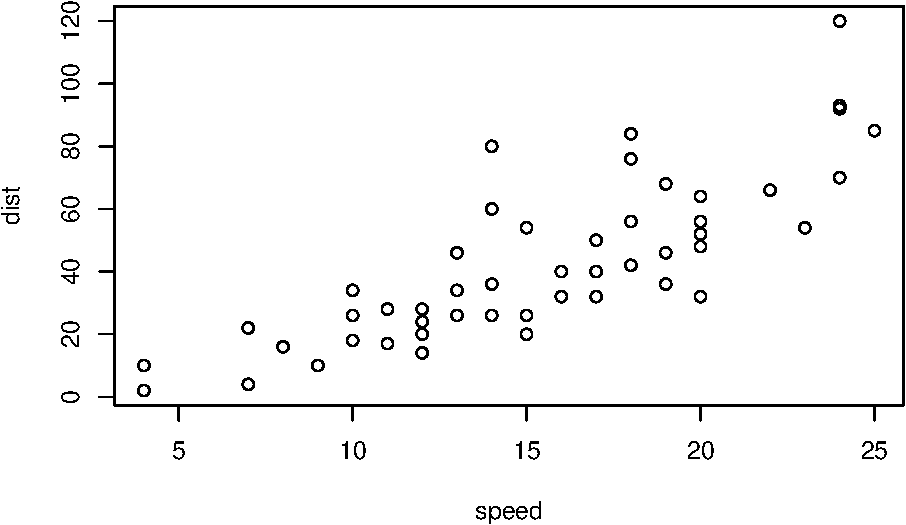
\includegraphics{snvdem24_files/figure-latex/unnamed-chunk-1-1.pdf}
\caption{A plot example}
\end{figure}

\hypertarget{table}{%
\subsection{Table}\label{table}}

Table example

\begin{longtable}[]{@{}rr@{}}
\toprule\noalign{}
speed & dist \\
\midrule\noalign{}
\endhead
\bottomrule\noalign{}
\endlastfoot
4 & 2 \\
4 & 10 \\
7 & 4 \\
7 & 22 \\
8 & 16 \\
9 & 10 \\
\end{longtable}

\hypertarget{various-guidelines}{%
\subsection{Various guidelines}\label{various-guidelines}}

\hypertarget{meth}{%
\section{Methods}\label{meth}}

Don't take any of these section titles seriously. They're just for
illustration.

\hypertarget{verify}{%
\section{Verifications}\label{verify}}

This section will be just long enough to illustrate what a full page of
text looks like, for margins and spacing.

\addtolength{\textheight}{.5in}%

The quick brown fox jumped over the lazy dog. The quick brown fox jumped
over the lazy dog. The quick brown fox jumped over the lazy dog. The
quick brown fox jumped over the lazy dog. \textbf{With this spacing we
have 25 lines per page.} The quick brown fox jumped over the lazy dog.
The quick brown fox jumped over the lazy dog. The quick brown fox jumped
over the lazy dog. The quick brown fox jumped over the lazy dog. The
quick brown fox jumped over the lazy dog.

The quick brown fox jumped over the lazy dog. The quick brown fox jumped
over the lazy dog. The quick brown fox jumped over the lazy dog. The
quick brown fox jumped over the lazy dog. The quick brown fox jumped
over the lazy dog. The quick brown fox jumped over the lazy dog. The
quick brown fox jumped over the lazy dog. The quick brown fox jumped
over the lazy dog. The quick brown fox jumped over the lazy dog. The
quick brown fox jumped over the lazy dog.

The quick brown fox jumped over the lazy dog. The quick brown fox jumped
over the lazy dog. The quick brown fox jumped over the lazy dog. The
quick brown fox jumped over the lazy dog. The quick brown fox jumped
over the lazy dog. The quick brown fox jumped over the lazy dog. The
quick brown fox jumped over the lazy dog. The quick brown fox jumped
over the lazy dog. The quick brown fox jumped over the lazy dog. The
quick brown fox jumped over the lazy dog.

\addtolength{\textheight}{-.3in}%

The quick brown fox jumped over the lazy dog. The quick brown fox jumped
over the lazy dog. The quick brown fox jumped over the lazy dog. The
quick brown fox jumped over the lazy dog. The quick brown fox jumped
over the lazy dog. The quick brown fox jumped over the lazy dog. The
quick brown fox jumped over the lazy dog. The quick brown fox jumped
over the lazy dog. The quick brown fox jumped over the lazy dog. The
quick brown fox jumped over the lazy dog.

The quick brown fox jumped over the lazy dog. The quick brown fox jumped
over the lazy dog. The quick brown fox jumped over the lazy dog. The
quick brown fox jumped over the lazy dog. The quick brown fox jumped
over the lazy dog. The quick brown fox jumped over the lazy dog. The
quick brown fox jumped over the lazy dog. The quick brown fox jumped
over the lazy dog. The quick brown fox jumped over the lazy dog. The
quick brown fox jumped over the lazy dog.

The quick brown fox jumped over the lazy dog. The quick brown fox jumped
over the lazy dog. The quick brown fox jumped over the lazy dog. The
quick brown fox jumped over the lazy dog. The quick brown fox jumped
over the lazy dog. The quick brown fox jumped over the lazy dog. The
quick brown fox jumped over the lazy dog. The quick brown fox jumped
over the lazy dog. The quick brown fox jumped over the lazy dog. The
quick brown fox jumped over the lazy dog.

The quick brown fox jumped over the lazy dog. The quick brown fox jumped
over the lazy dog. The quick brown fox jumped over the lazy dog. The
quick brown fox jumped over the lazy dog. The quick brown fox jumped
over the lazy dog. The quick brown fox jumped over the lazy dog. The
quick brown fox jumped over the lazy dog. The quick brown fox jumped
over the lazy dog. The quick brown fox jumped over the lazy dog. The
quick brown fox jumped over the lazy dog.

The quick brown fox jumped over the lazy dog. The quick brown fox jumped
over the lazy dog. The quick brown fox jumped over the lazy dog. The
quick brown fox jumped over the lazy dog. The quick brown fox jumped
over the lazy dog. The quick brown fox jumped over the lazy dog. The
quick brown fox jumped over the lazy dog. The quick brown fox jumped
over the lazy dog. The quick brown fox jumped over the lazy dog. The
quick brown fox jumped over the lazy dog.

The quick brown fox jumped over the lazy dog. The quick brown fox jumped
over the lazy dog. The quick brown fox jumped over the lazy dog. The
quick brown fox jumped over the lazy dog. The quick brown fox jumped
over the lazy dog. The quick brown fox jumped over the lazy dog. The
quick brown fox jumped over the lazy dog. The quick brown fox jumped
over the lazy dog. The quick brown fox jumped over the lazy dog. The
quick brown fox jumped over the lazy dog.

The quick brown fox jumped over the lazy dog. The quick brown fox jumped
over the lazy dog. The quick brown fox jumped over the lazy dog. The
quick brown fox jumped over the lazy dog. The quick brown fox jumped
over the lazy dog. The quick brown fox jumped over the lazy dog. The
quick brown fox jumped over the lazy dog. The quick brown fox jumped
over the lazy dog. The quick brown fox jumped over the lazy dog. The
quick brown fox jumped over the lazy dog.

The quick brown fox jumped over the lazy dog. The quick brown fox jumped
over the lazy dog. The quick brown fox jumped over the lazy dog. The
quick brown fox jumped over the lazy dog.

\hypertarget{conc}{%
\section{Conclusion}\label{conc}}

\bigskip

\begin{center}
\textbf{SUPPLEMENTARY MATERIAL}

\end{center}

\begin{quote}
Use \href{https://pandoc.org/MANUAL.html\#definition-lists}{definition
list syntax} in this part
\end{quote}

\begin{description}
\tightlist
\item[Title:]
Brief description. (file type)
\item[R-package for MYNEW routine:]
R-package \textbf{MYNEW} containing code to perform the diagnostic
methods described in the article. The package also contains all datasets
used as examples in the article. (GNU zipped tar file)
\item[HIV data set:]
Data set used in the illustration of MYNEW method in
Section\textasciitilde{} 3.2. (.txt file)
\end{description}

\hypertarget{bibliography.}{%
\section{Bibliography.}\label{bibliography.}}

Using \texttt{natbib} is the default with this format, using
\texttt{plain.bst} by default on the template, and \texttt{apalike.bst}
in this Rmd skeleton. Chante to your preference using the
\texttt{biblio-style} in YAML

\bibliographystyle{apalike}
\bibliography{}



\end{document}
